\chapter{Graph Signal Processing of Brain Connectome Networks}
\label{chap:gsp_connectome} % chktex 24

This chapter develops the graph signal processing (GSP) framework used to analyze atlas-based brain connectomes and to train a geometric deep learning model for disease prediction under an explicit smoothness prior. The central modeling principle is that the predictive representation should remain \emph{task-specific} while also being \emph{regularized on the graph}. Concretely, the model parameters are learned by minimizing a prediction loss together with a graph smoothness penalty derived from Dirichlet energy. This chapter therefore unifies four threads:
\begin{enumerate}[label=(\roman*)] % chktex 36
    \item construction of a shared brain graph from anatomical regions,
    \item representation of regional measurements as graph signals,
    \item spectral and wavelet characterization of disease-related deviations, and
    \item supervised learning with a prediction objective regularized by graph smoothness.
\end{enumerate}

The chapter is organized as follows. Section~\ref{sec:ch4_intro} motivates the GSP viewpoint. Section~\ref{sec:ch4_graph_construction} defines the graph and associated operators. Section~\ref{sec:ch4_signals} introduces regional measurements as signals over nodes. Section~\ref{sec:ch4_spectral} develops spectral graph analysis, including the graph Fourier transform, spectral energy, spectral centroid, and spectral entropy. Section~\ref{sec:ch4_wavelets} presents multiscale graph wavelets. Section~\ref{sec:ch4_diffusion} interprets smoothness via heat diffusion and Dirichlet energy. Section~\ref{sec:ch4_gdl} formulates the geometric deep learning model, its message passing rule, and the training objective. Section~\ref{sec:ch4_biomarkers} summarizes spectral biomarkers of disease. Section~\ref{sec:ch4_robustness} comments on stability and robustness, and Section~\ref{sec:ch4_results_overview} integrates the experimental evidence.

\section{Introduction}
\label{sec:ch4_intro} % chktex 24

Brain imaging data are naturally structured: measurements are not independent across space, but are constrained by anatomy, functional relationships, and long-range organization. When regional quantities are aggregated over a cortical atlas, each brain scan may be described as a signal over a set of graph nodes, where nodes correspond to regions of interest (ROIs) and edges encode inter-regional affinity. This representation makes GSP a natural mathematical language for studying how disease perturbs spatial organization.

Let
\[
G = (V,E,W)
\]
denote an undirected weighted graph with node set \(V=\{1,\dots,N\}\), edge set \(E\), and symmetric weighted adjacency matrix \(W \in \mathbb{R}^{N\times N}\), where \(W_{ij} \ge 0\). For each subject \(s\), an imaging-derived regional measurement is represented as a graph signal
\[
x^{(s)} \in \mathbb{R}^{N},
\]
whose \(i\)-th entry is the mean signal value in region \(i\). A disease classifier then maps the graph signal (and optionally graph structure) to a label
\[
y^{(s)} \in \{0,1\},
\]
with \(y^{(s)}=1\) representing GBM and \(y^{(s)}=0\) representing healthy tissue.

The key idea adopted here is that biologically meaningful graph signals often exhibit \emph{piecewise smoothness}: neighboring regions tend to have related values unless disrupted by pathology. This motivates regularizing the learned predictive representation using graph Dirichlet energy. The resulting objective balances prediction fidelity against structural smoothness:
\begin{equation}
\label{eq:main_objective_intro}
\mathcal{L}_{\text{total}}
=
\mathcal{L}_{\text{pred}}
+
\lambda \,\mathcal{L}_{\text{smooth}},
\end{equation}
where \(\mathcal{L}_{\text{pred}}\) is task-specific and \(\mathcal{L}_{\text{smooth}}\) is a smoothness penalty derived from graph Dirichlet energy, with regularization weight \(\lambda>0\).

This formulation is consistent across all analyses in the chapter: the spectrum, graph wavelets, and smoothness measures are used both as descriptive tools and as principled regularizers in the supervised learning problem.

\section{Construction of the Brain Connectome Graph}
\label{sec:ch4_graph_construction} % chktex 24

\subsection{Network Definition}

A common atlas provides a shared node set across subjects. In this work, the Harvard--Oxford cortical atlas is used to define \(N=48\) cortical ROIs, giving a fixed graph topology for all subjects. Let the node set be % chktex 8
\[
V=\{1,\dots,48\}.
\]
An undirected edge \((i,j)\in E\) is included when regions \(i\) and \(j\) are considered anatomically or statistically connected in the shared reference graph. The graph is represented by its weighted adjacency matrix \(W\), degree matrix \(D\), and graph Laplacian \(L\):
\begin{align}
W_{ij} &= W_{ji} \ge 0,\\
D_{ii} &= \sum_{j=1}^{N} W_{ij},\\
L &= D - W.
\end{align}
Because node degrees may vary, the normalized Laplacian is also useful:
\begin{equation}
\label{eq:normalized_laplacian}
L_{\mathrm{sym}}
=
I - D^{-1/2} W D^{-1/2}.
\end{equation}
The normalized version permits comparison across regions with different connectivity levels and is particularly convenient for spectral analysis and graph convolutions.

\subsection{Atlas and Spatial Registration}

The atlas-based construction pipeline is illustrated in Figures~\ref{fig:mni_atlas}--\ref{fig:tumor_mask_alignment}. The MNI152 template provides the common reference space, the Harvard--Oxford atlas provides ROI labels, and subject-level MRI/tumor masks are mapped into this space so that node-wise quantities can be computed consistently across the cohort. % chktex 8

\begin{figure}[H]
    \centering
    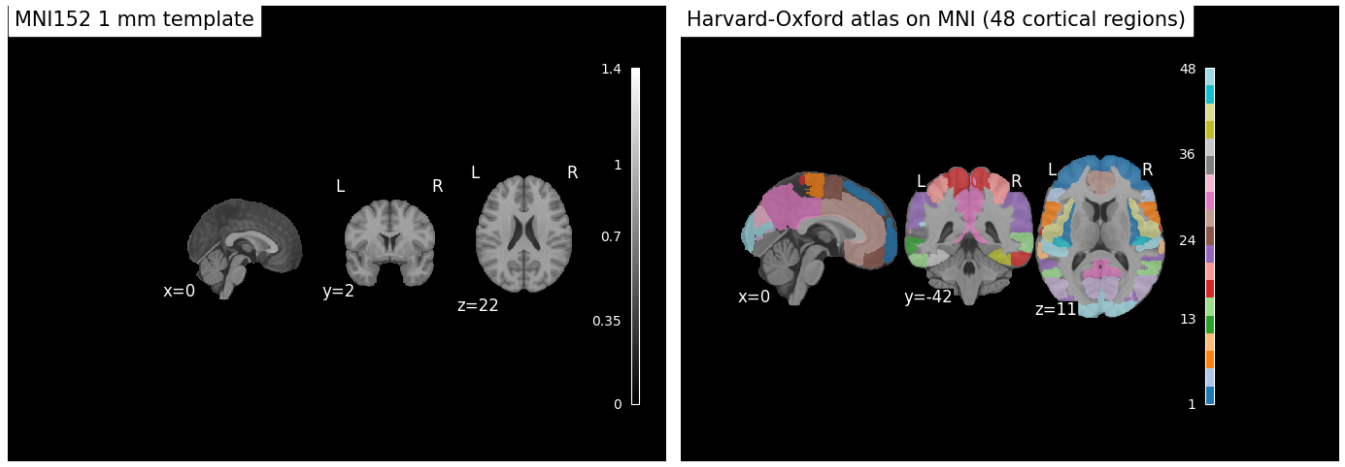
\includegraphics[width=0.98\textwidth]{chapter4_assets/harvard-oxford-atlas.png}
    \caption{Reference space and atlas definition. Left: MNI152 1\,mm template. Right: Harvard--Oxford atlas projected onto MNI space with 48 cortical regions. This atlas defines the graph nodes used throughout the chapter.} % chktex 8
    \label{fig:mni_atlas} % chktex 24
\end{figure}

\begin{figure}[H]
    \centering
    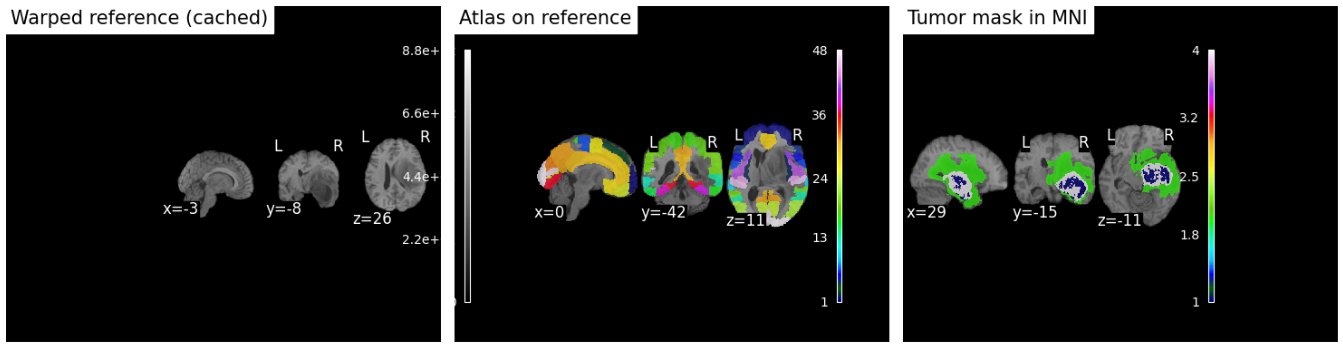
\includegraphics[width=0.98\textwidth]{chapter4_assets/tumor-mask-comparison.png}
    \caption{Registration and atlas alignment workflow. The reference image, atlas labels, and tumor mask are shown in common space, enabling atlas-wise aggregation of tumor burden and image-derived regional signals.}
    \label{fig:tumor_mask_alignment} % chktex 24
\end{figure}

Figure~\ref{fig:subject_mri_example} shows a representative warped reference image for a GBM subject. After registration, each atlas node receives a region-level summary statistic, such as the mean T1 intensity or the fraction of voxels covered by tumor.

\begin{figure}[H]
    \centering
    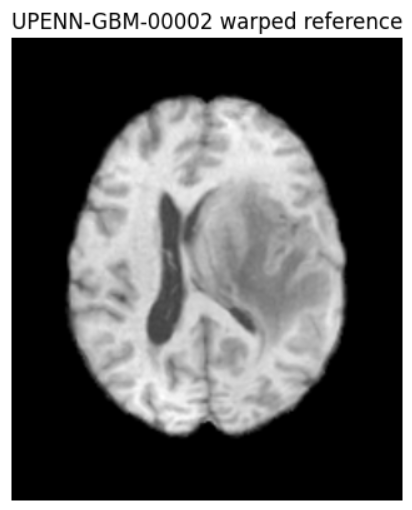
\includegraphics[width=0.35\textwidth]{chapter4_assets/example-brain-mri-GBM.png}
    \caption{Example subject in aligned space. A representative GBM case is shown after warping into the common reference frame used for atlas aggregation.}
    \label{fig:subject_mri_example} % chktex 24
\end{figure}

\subsection{Descriptive Topology of the Shared Connectome}

Before learning on graph signals, it is useful to characterize the topology of the shared graph itself. Figure~\ref{fig:connectome_descriptive_statistics} summarizes the degree distribution, clustering coefficient distribution, betweenness centrality distribution, and graph visualizations colored by several node-level attributes. These descriptive measures provide intuition for where smoothness penalties will be strongest and where perturbations may propagate.

\begin{figure}[H]
    \centering
    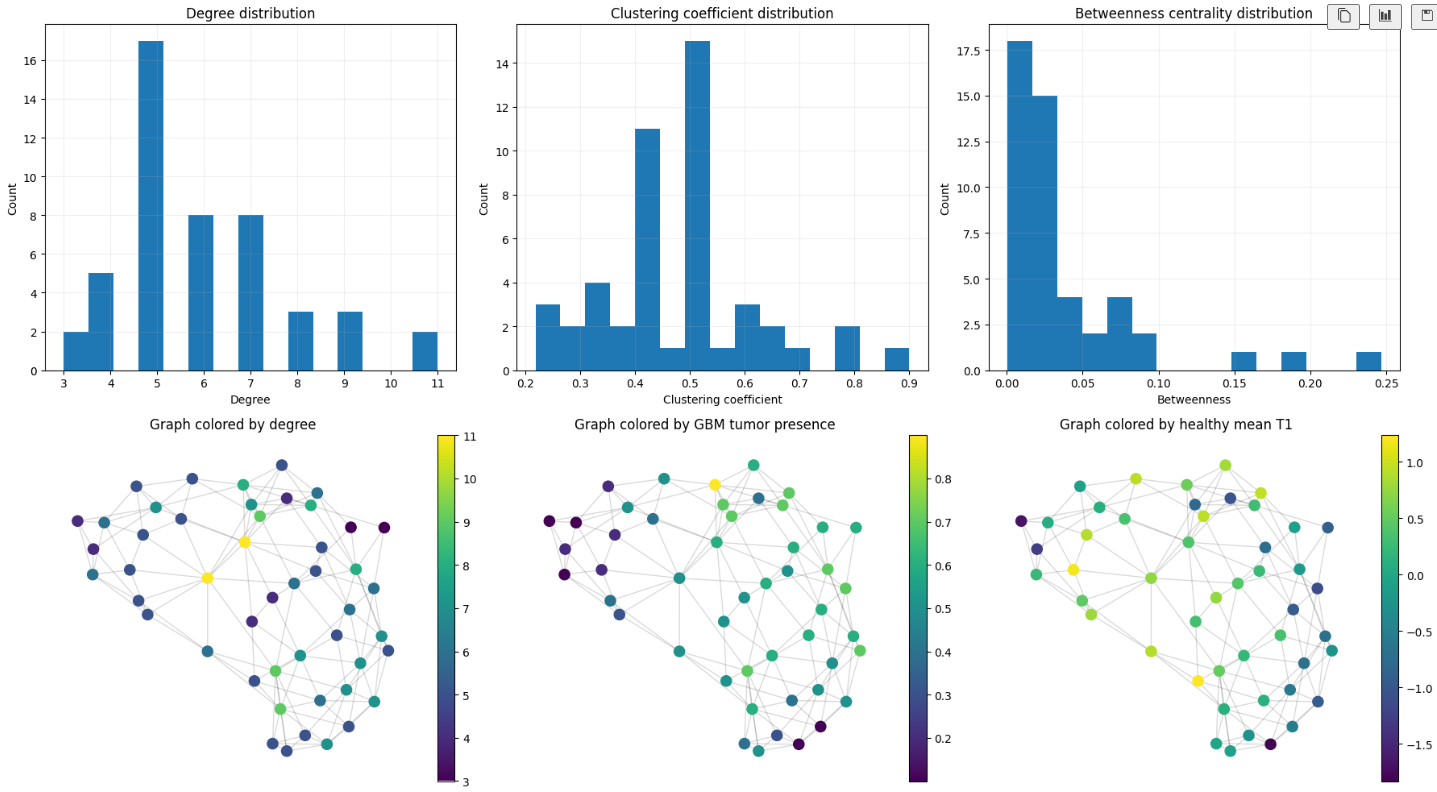
\includegraphics[width=\textwidth]{chapter4_assets/connectome-by-descriptive-stat.png}
    \caption{Descriptive graph statistics and graph visualizations for the shared 48-node connectome. Top row: distributions of degree, clustering coefficient, and betweenness centrality. Bottom row: the same graph colored by degree, average GBM tumor presence, and average healthy mean T1 signal.}
    \label{fig:connectome_descriptive_statistics} % chktex 24
\end{figure}

If \(d_i\) is the degree of node \(i\), the average degree is
\begin{equation}
\bar d = \frac{1}{N}\sum_{i=1}^{N} d_i.
\end{equation}
The local clustering coefficient of node \(i\) may be written as
\begin{equation}
C_i = \frac{2T_i}{d_i(d_i-1)},
\end{equation}
where \(T_i\) is the number of triangles through node \(i\). Betweenness centrality quantifies how frequently a node lies on shortest paths:
\begin{equation}
B_i = \sum_{\substack{s\neq i\neq t\\ s<t}} \frac{\sigma_{st}(i)}{\sigma_{st}},
\end{equation}
where \(\sigma_{st}\) is the number of shortest paths from \(s\) to \(t\) and \(\sigma_{st}(i)\) counts those passing through \(i\).

These graph properties matter because a smoothness penalty of the form \(f^\top L f\) penalizes differences across edges; nodes with many strong incident edges contribute more strongly to the total regularization.

\section{Brain Measurements as Graph Signals}
\label{sec:ch4_signals} % chktex 24

\subsection{Regional Signal Definition}

Given a subject-level image \(I^{(s)}(\mathbf{r})\) in common space and an atlas region \(\Omega_i\), a node-wise regional summary signal is defined as
\begin{equation}
x_i^{(s)}
=
\frac{1}{|\Omega_i|}
\sum_{\mathbf{r}\in\Omega_i} I^{(s)}(\mathbf{r}),
\end{equation}
or, in continuous notation,
\begin{equation}
x_i^{(s)}
=
\frac{1}{\mu(\Omega_i)} \int_{\Omega_i} I^{(s)}(\mathbf{r})\,d\mathbf{r}.
\end{equation}
Stacking across all nodes yields the graph signal \(x^{(s)} \in \mathbb{R}^{N}\).

Two particularly important signals in this chapter are:
\begin{enumerate}[label=(\alph*)] % chktex 36
    \item the mean T1 signal \(x_{\mathrm{t1}}^{(s)}\), and
    \item the tumor burden signal \(x_{\mathrm{tumor}}^{(s)}\), where
    \begin{equation}
    x^{(s)}_{\mathrm{tumor},i}
    =
    \frac{1}{|\Omega_i|}
    \sum_{\mathbf{r}\in\Omega_i} M^{(s)}(\mathbf{r}),
    \end{equation}
    with \(M^{(s)}(\mathbf{r})\in\{0,1\}\) the tumor mask.
\end{enumerate}

The tumor burden by atlas node for a representative case is shown in Figure~\ref{fig:tumor_by_node}, revealing spatially nonuniform disease distribution over the connectome.

\begin{figure}[H]
    \centering
    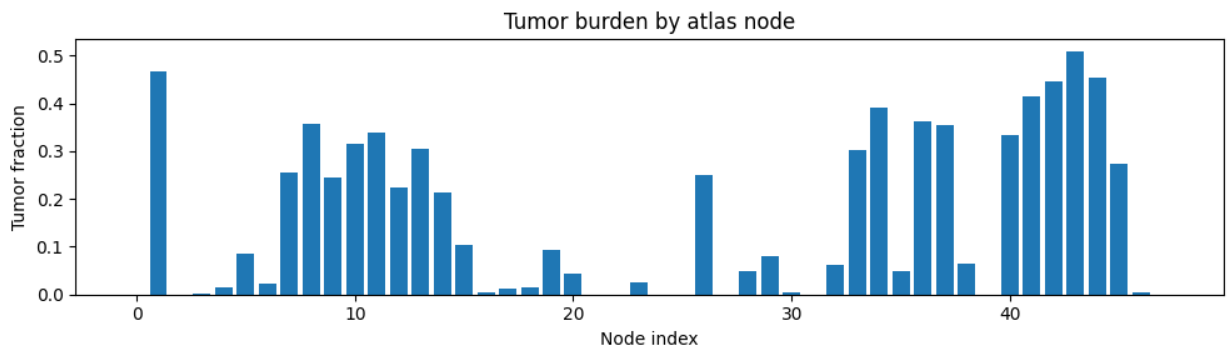
\includegraphics[width=0.9\textwidth]{chapter4_assets/tumor-by-atlas-node-main.png}
    \caption{Tumor burden by atlas node for a representative GBM subject. The node-wise tumor fraction defines a graph signal that can be analyzed spectrally and spatially.}
    \label{fig:tumor_by_node} % chktex 24
\end{figure}

\subsection{Cohort Mean Signals and Disease-Related Spatial Contrast}

Let \(\mathcal{S}_{\mathrm{GBM}}\) and \(\mathcal{S}_{\mathrm{H}}\) denote the GBM and healthy cohorts. Their mean signals are
\begin{align}
\bar x_{\mathrm{GBM}} &= \frac{1}{|\mathcal{S}_{\mathrm{GBM}}|}\sum_{s\in\mathcal{S}_{\mathrm{GBM}}} x^{(s)},\\
\bar x_{\mathrm{H}} &= \frac{1}{|\mathcal{S}_{\mathrm{H}}|}\sum_{s\in\mathcal{S}_{\mathrm{H}}} x^{(s)}.
\end{align}
A natural disease contrast is then
\begin{equation}
\Delta x = \bar x_{\mathrm{GBM}} - \bar x_{\mathrm{H}}.
\end{equation}

Figure~\ref{fig:mean_signal_graphs} visualizes the mean GBM signal, mean healthy signal, and the cohort-level difference over the shared connectome. The disease effect is not spatially uniform; instead it is concentrated over subsets of regions, motivating graph-based multiscale analysis.

\begin{figure}[H]
    \centering
    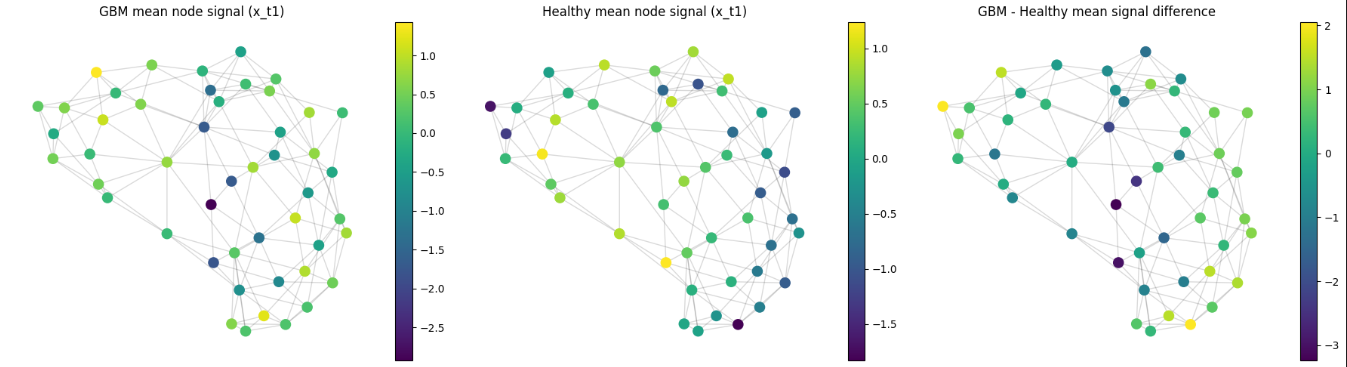
\includegraphics[width=\textwidth]{chapter4_assets/disease-normal-delta-connectome.png}
    \caption{Cohort mean graph signals and their difference. Left: mean GBM node signal. Middle: mean healthy node signal. Right: GBM minus healthy mean signal. Disease-related deviations are spatially structured over the graph rather than randomly distributed.}
    \label{fig:mean_signal_graphs} % chktex 24
\end{figure}

Figure~\ref{fig:gbm_mean_presence} similarly shows the average tumor presence over the shared graph, providing a biologically interpretable disease burden map.

\begin{figure}[H]
    \centering
    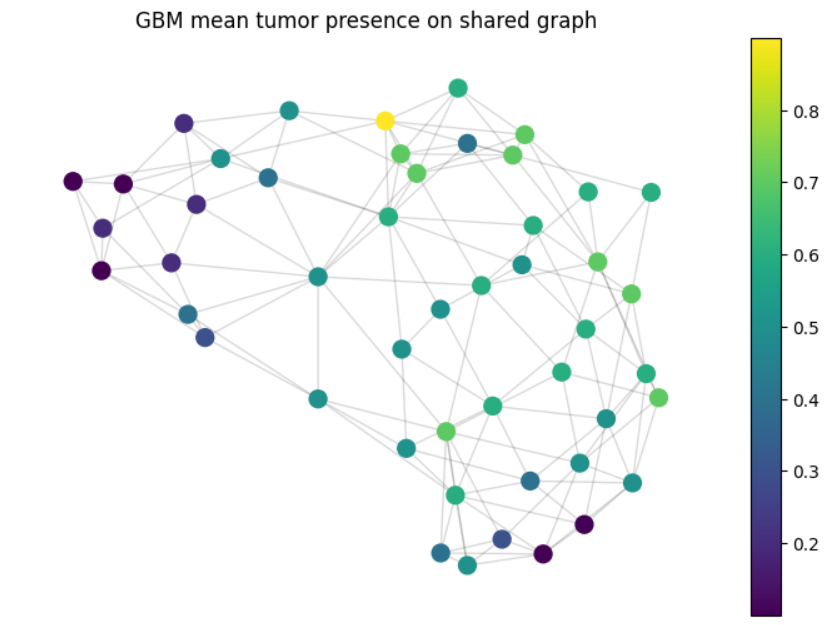
\includegraphics[width=0.62\textwidth]{chapter4_assets/gbm-mean-presence.png}
    \caption{Average GBM tumor presence projected onto the shared graph. This cohort-level map indicates which atlas nodes are most frequently involved by tumor across GBM subjects.}
    \label{fig:gbm_mean_presence} % chktex 24
\end{figure}

\section{Spectral Graph Analysis of Brain Signals}
\label{sec:ch4_spectral} % chktex 24

\subsection{Graph Fourier Transform}

The graph Laplacian \(L\) is real symmetric and admits the eigendecomposition
\begin{equation}
\label{eq:laplacian_eigendecomp}
L = U \Lambda U^\top,
\end{equation}
where
\[
U = [u_1,\dots,u_N], \qquad
\Lambda = \mathrm{diag}(\lambda_1,\dots,\lambda_N),
\]
with
\[
0=\lambda_1 \le \lambda_2 \le \cdots \le \lambda_N.
\]
The graph Fourier transform (GFT) of a signal \(x\in\mathbb{R}^N\) is defined by
\begin{equation}
\hat x = U^\top x,
\end{equation}
with inverse transform
\begin{equation}
x = U \hat x = \sum_{k=1}^{N} \hat x_k u_k.
\end{equation}
Low graph frequencies correspond to Laplacian eigenvectors with small eigenvalues and vary slowly over strongly connected regions, whereas high graph frequencies oscillate more sharply across neighboring nodes.

\subsection{Dirichlet Energy and Spectral Smoothness}

A central quantity in this chapter is the graph Dirichlet energy:
\begin{equation}
\label{eq:dirichlet_energy}
\mathcal{E}(x)
=
x^\top L x
=
\frac{1}{2}\sum_{i=1}^{N}\sum_{j=1}^{N} W_{ij}(x_i-x_j)^2. % chktex 3
\end{equation}
Equation~\eqref{eq:dirichlet_energy} gives two equivalent interpretations:
\begin{enumerate}[label=(\arabic*)] % chktex 36
    \item in the vertex domain, it penalizes edge-wise disagreement;
    \item in the spectral domain, it weights energy by graph frequency.
\end{enumerate}
Indeed, using \(L=U\Lambda U^\top\),
\begin{equation}
\mathcal{E}(x)
=
x^\top U\Lambda U^\top x
=
\hat x^\top \Lambda \hat x
=
\sum_{k=1}^{N} \lambda_k |\hat x_k|^2.
\end{equation}
Thus a signal is smooth if most of its spectral mass lies at low eigenvalues.

\subsection{Spectral Energy Distribution}

Let \(\hat x_k\) denote the \(k\)-th GFT coefficient. The spectral power at graph frequency \(\lambda_k\) is defined by
\begin{equation}
P_k = |\hat x_k|^2.
\end{equation}
The total spectral energy is
\begin{equation}
E_{\mathrm{tot}} = \sum_{k=1}^{N} P_k = \|x\|_2^2.
\end{equation}
To study disease-related differences, the mean spectra of the GBM and healthy cohorts are compared in Figure~\ref{fig:cancer_vs_normal_spectra}. The healthy cohort shows relatively stronger content in a broader range of graph frequencies, while the GBM cohort exhibits a different distribution of spectral power, especially in lower-to-mid frequencies.

\begin{figure}[H]
    \centering
    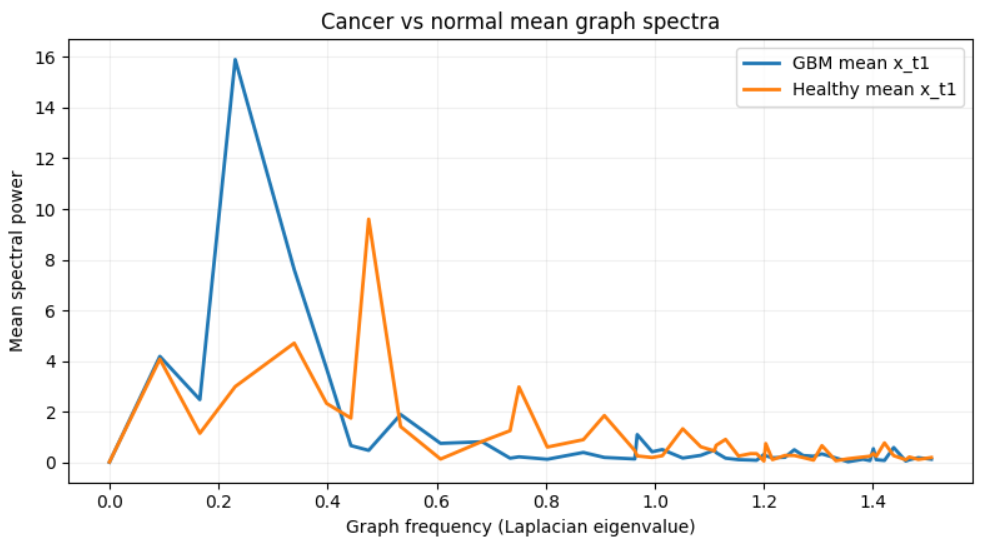
\includegraphics[width=0.78\textwidth]{chapter4_assets/cancervsnormal-spectra.png}
    \caption{Mean graph spectra for GBM and healthy cohorts. The spectra are plotted as spectral power versus graph frequency (Laplacian eigenvalue), highlighting disease-related redistribution of energy across graph harmonics.}
    \label{fig:cancer_vs_normal_spectra} % chktex 24
\end{figure}

A representative average GBM tumor spectrum is shown in Figure~\ref{fig:avg_gbm_tumor_spectrum}. The marked high-frequency cutoff illustrates a convenient operational partition between low-frequency and high-frequency graph content.

\begin{figure}[H]
    \centering
    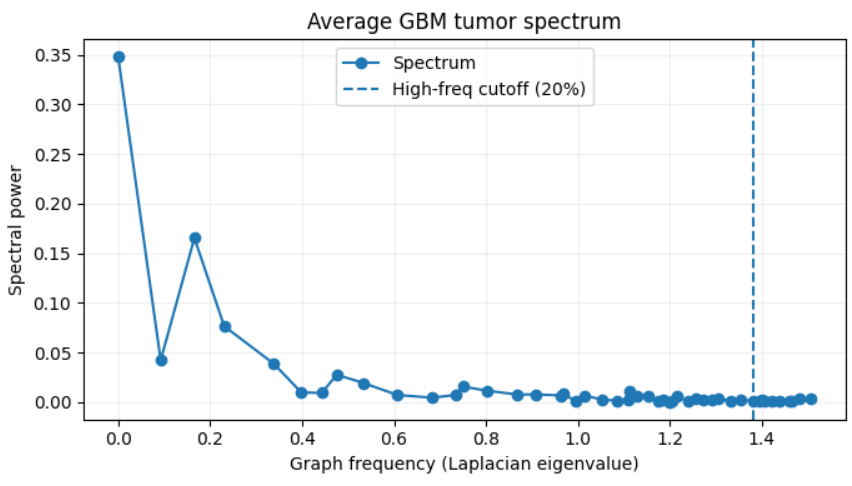
\includegraphics[width=0.74\textwidth]{chapter4_assets/average-GBM-tumor-spectrum.png}
    \caption{Average GBM tumor spectrum. The dashed vertical line indicates a high-frequency cutoff (here shown at the upper 20\% of graph frequencies), which is later used to define high-frequency spectral energy.}
    \label{fig:avg_gbm_tumor_spectrum} % chktex 24
\end{figure}

\subsection{Spectral Biomarkers}

Several scalar spectral descriptors are useful for summarizing graph signals.

\paragraph{Low-frequency energy.}
Let \(\mathcal{K}_{\mathrm{low}}\) denote an index set of low graph frequencies. Then
\begin{equation}
E_{\mathrm{low}}(x)
=
\sum_{k\in\mathcal{K}_{\mathrm{low}}} |\hat x_k|^2.
\end{equation}

\paragraph{High-frequency energy.}
Similarly, for \(\mathcal{K}_{\mathrm{high}}\),
\begin{equation}
E_{\mathrm{high}}(x)
=
\sum_{k\in\mathcal{K}_{\mathrm{high}}} |\hat x_k|^2.
\end{equation}
Larger \(E_{\mathrm{high}}\) indicates sharper spatial variation and reduced smoothness.

\paragraph{Spectral centroid.}
The spectral centroid summarizes where the signal is centered in graph frequency:
\begin{equation}
\label{eq:spectral_centroid}
C_{\mathrm{spec}}(x)
=
\frac{\sum_{k=1}^{N} \lambda_k |\hat x_k|^2}
{\sum_{k=1}^{N} |\hat x_k|^2}.
\end{equation}
This is the energy-weighted average graph frequency. Higher values imply a shift toward less smooth components.

\paragraph{Spectral entropy.}
Define normalized spectral weights
\begin{equation}
p_k = \frac{|\hat x_k|^2}{\sum_{\ell=1}^{N} |\hat x_\ell|^2}.
\end{equation}
Then the spectral entropy is
\begin{equation}
\label{eq:spectral_entropy}
H_{\mathrm{spec}}(x)
=
-\sum_{k=1}^{N} p_k \log p_k.
\end{equation}
Higher entropy indicates a more diffuse spectral distribution.

Figure~\ref{fig:mean_spectral_metrics} summarizes mean spectral descriptors by cohort. The healthy cohort tends to exhibit larger high-frequency energy, larger centroid, and larger entropy than the GBM tumor signal, suggesting that the tumor burden signal is comparatively more concentrated in low graph frequencies, whereas healthy T1-related variation is more broadly distributed across harmonics.

\begin{figure}[H]
    \centering
    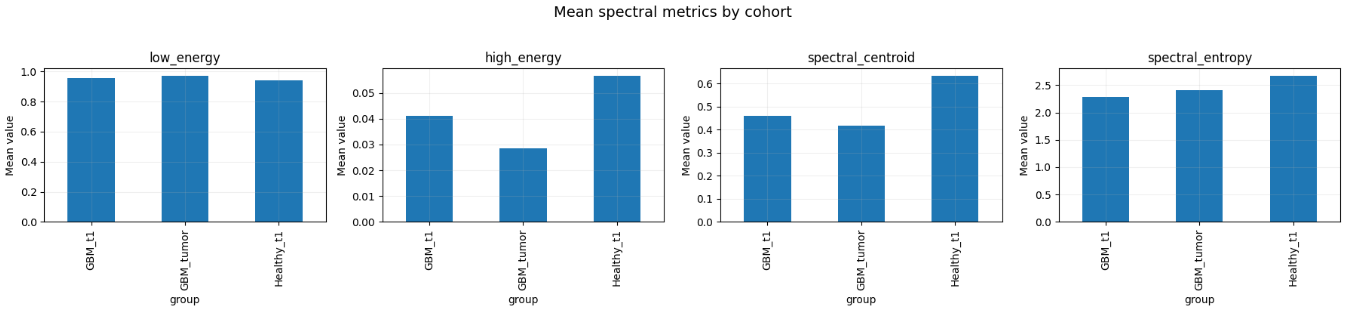
\includegraphics[width=\textwidth]{chapter4_assets/spectral_metrics.png}
    \caption{Mean spectral metrics by cohort: low-frequency energy, high-frequency energy, spectral centroid, and spectral entropy. These compact descriptors summarize the organization of graph signal energy across the spectrum.}
    \label{fig:mean_spectral_metrics} % chktex 24
\end{figure}

The distributional comparisons are shown in Figures~\ref{fig:centroid_box}, \ref{fig:highfreq_box}, \ref{fig:entropy_box}, \ref{fig:centroid_box_all}, and \ref{fig:highfreq_box_all}. They highlight that graph spectral measures can separate tissue states at the cohort level. % chktex 2

\begin{figure}[H]
    \centering
    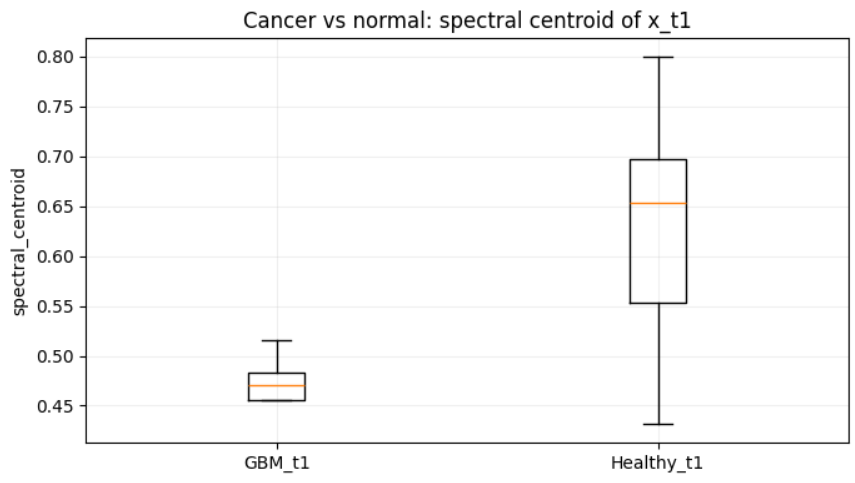
\includegraphics[width=0.58\textwidth]{chapter4_assets/cancervsnormal-centroid-t1.png}
    \caption{Cancer versus normal comparison of spectral centroid for the T1 signal. The healthy cohort exhibits a higher centroid, consistent with stronger energy at higher graph frequencies.}
    \label{fig:centroid_box} % chktex 24
\end{figure}

\begin{figure}[H]
    \centering
    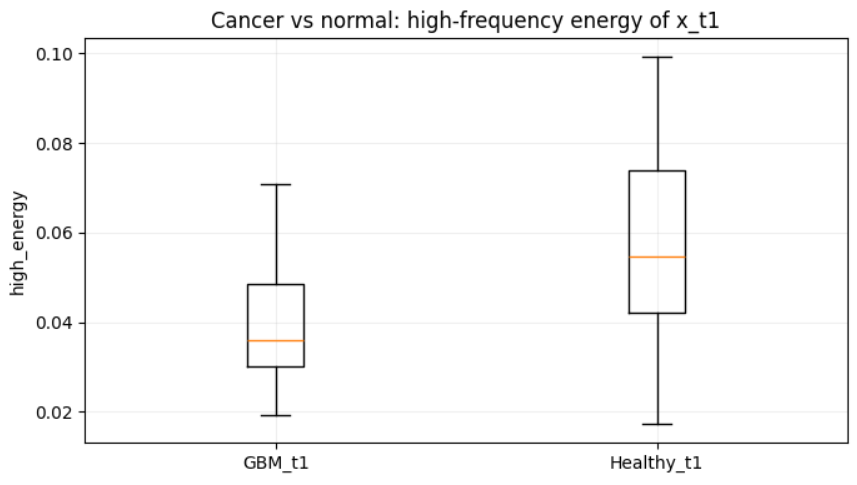
\includegraphics[width=0.58\textwidth]{chapter4_assets/cancervsnormal_t1_highfreq.png}
    \caption{Cancer versus normal comparison of high-frequency graph spectral energy for the T1 signal. Healthy signals exhibit higher high-frequency energy than GBM signals in this dataset.}
    \label{fig:highfreq_box} % chktex 24
\end{figure}

\begin{figure}[H]
    \centering
    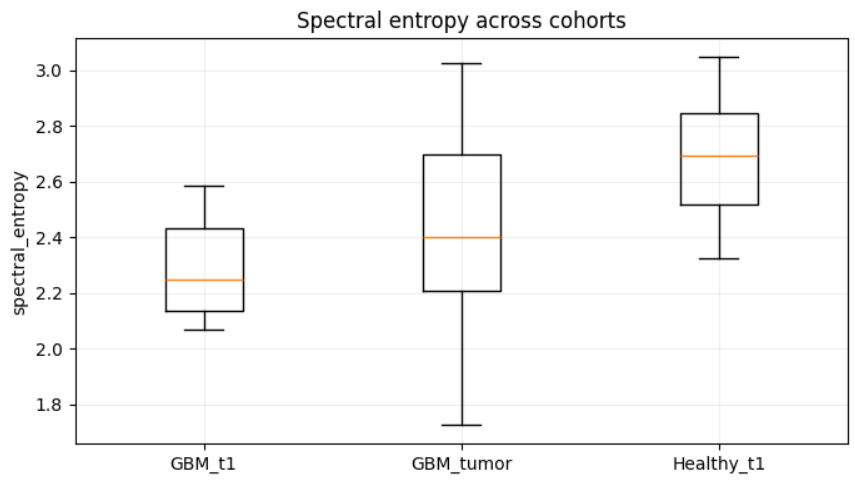
\includegraphics[width=0.68\textwidth]{chapter4_assets/spectral-entropy-box.png}
    \caption{Spectral entropy across cohorts. Healthy signals show the broadest and highest-entropy spectral distribution, while GBM-related signals are relatively more concentrated.}
    \label{fig:entropy_box} % chktex 24
\end{figure}

\begin{figure}[H]
    \centering
    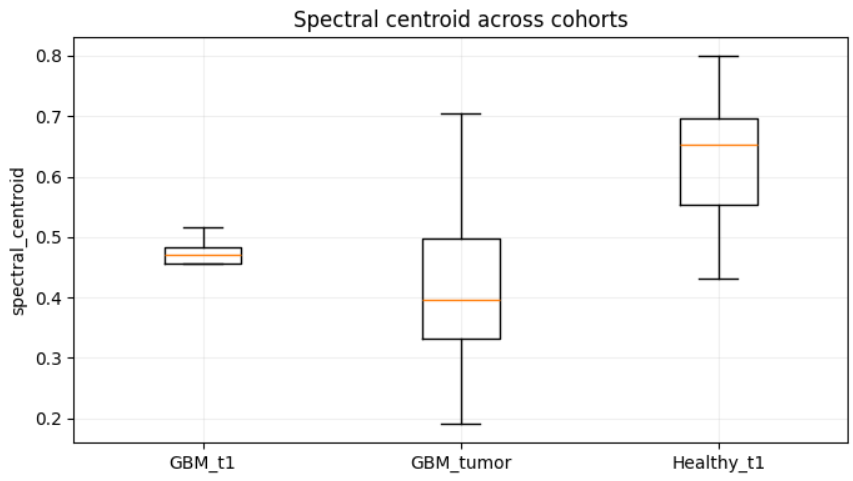
\includegraphics[width=0.68\textwidth]{chapter4_assets/spectral-centroid-box.png}
    \caption{Spectral centroid across cohorts. The healthy cohort tends to occupy higher graph frequencies on average than the disease-related graph signals.}
    \label{fig:centroid_box_all} % chktex 24
\end{figure}

\begin{figure}[H]
    \centering
    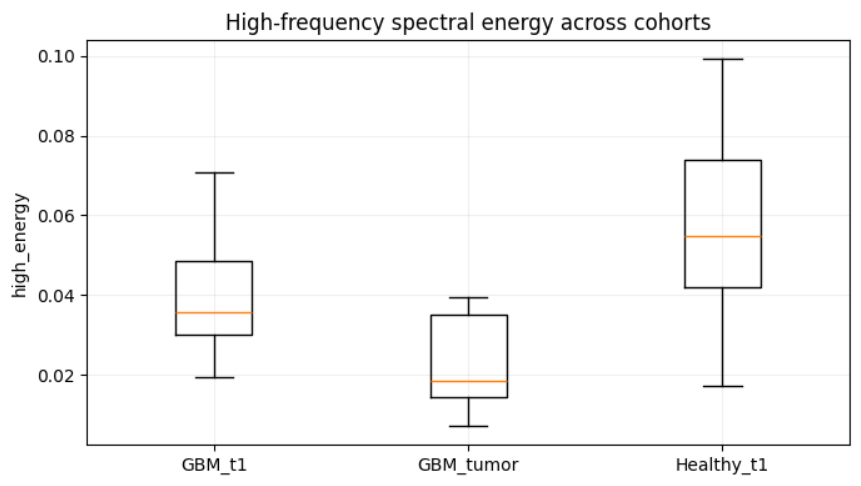
\includegraphics[width=0.68\textwidth]{chapter4_assets/spectral-energy-box1.png}
    \caption{High-frequency spectral energy across cohorts. The healthy cohort shows the largest high-frequency energy, while the GBM tumor signal is more heavily concentrated in lower frequencies.}
    \label{fig:highfreq_box_all} % chktex 24
\end{figure}

\subsection{Summary Table of Spectral Descriptors}

Table~\ref{tab:spectral_metrics_interpretation} summarizes the interpretation of the principal spectral biomarkers used in this chapter.

\begin{table}[H]
    \centering
    \caption{Spectral biomarkers and their interpretation in the connectome graph setting.}
    \label{tab:spectral_metrics_interpretation} % chktex 24
    \begin{tabular}{p{3.0cm} p{4.3cm} p{7.0cm}}
        \toprule
        \textbf{Metric} & \textbf{Formula} & \textbf{Interpretation} \\
        \midrule
        Low-frequency energy &
        \(E_{\mathrm{low}}=\sum_{k\in\mathcal{K}_{\mathrm{low}}} |\hat x_k|^2\) &
        Measures signal power concentrated in smooth graph harmonics. Larger values imply stronger global smoothness and coherent regional structure. \\
        \addlinespace
        High-frequency energy &
        \(E_{\mathrm{high}}=\sum_{k\in\mathcal{K}_{\mathrm{high}}} |\hat x_k|^2\) &
        Measures signal power concentrated in rapidly varying graph harmonics. Larger values imply sharper regional contrast and less smoothness. \\
        \addlinespace
        Spectral centroid &
        \(C_{\mathrm{spec}}=\dfrac{\sum_k \lambda_k |\hat x_k|^2}{\sum_k |\hat x_k|^2}\) &
        Energy-weighted average graph frequency. Higher values indicate the spectrum is shifted toward less smooth components. \\
        \addlinespace
        Spectral entropy &
        \(H_{\mathrm{spec}}=-\sum_k p_k\log p_k\) &
        Quantifies how diffuse the spectrum is. Higher values indicate more distributed energy across modes rather than concentration in a few components. \\
        \bottomrule
    \end{tabular}
\end{table}

\section{Graph Wavelet Analysis}
\label{sec:ch4_wavelets} % chktex 24

Spectral descriptors summarize overall distribution of graph frequency content, but they do not explicitly preserve localization in both vertex and scale domains. Graph wavelets address this by defining multiscale filters on the Laplacian spectrum.

\subsection{Spectral Graph Wavelets}

Let \(g(\cdot)\) be a spectral kernel. A graph wavelet operator at scale \(\tau>0\) is
\begin{equation}
T_{g}^{(\tau)} = g(\tau L) = U\,g(\tau \Lambda)\,U^\top,
\end{equation}
where
\[
g(\tau \Lambda) = \mathrm{diag}\!\big(g(\tau\lambda_1),\dots,g(\tau\lambda_N)\big).
\]
Applying this operator to a graph signal \(x\) gives the scale-dependent wavelet coefficients
\begin{equation}
w^{(\tau)} = T_{g}^{(\tau)}x.
\end{equation}
The coefficient at node \(i\) and scale \(\tau\) is
\begin{equation}
w_i^{(\tau)} = \big[T_{g}^{(\tau)}x\big]_i. % chktex 3
\end{equation}
For heat-kernel-style diffusion wavelets one may use
\begin{equation}
g(\tau\lambda)=e^{-\tau\lambda},
\end{equation}
where small \(\tau\) emphasizes finer detail and large \(\tau\) emphasizes coarser smoothing.

\subsection{Multiscale Energy}

The wavelet energy at scale \(\tau\) is
\begin{equation}
E_{\mathrm{wav}}(\tau;x) = \|w^{(\tau)}\|_2^2.
\end{equation}
Comparing this quantity across cohorts reveals how disease-related signals organize across scales. Figure~\ref{fig:wavelet_boxplots} shows multiscale graph wavelet energy at \(\tau=1,5,10,20\). Healthy T1 signals exhibit markedly larger wavelet energy at smaller and intermediate scales, while the GBM tumor signal remains comparatively small and compressed.

\begin{figure}[H]
    \centering
    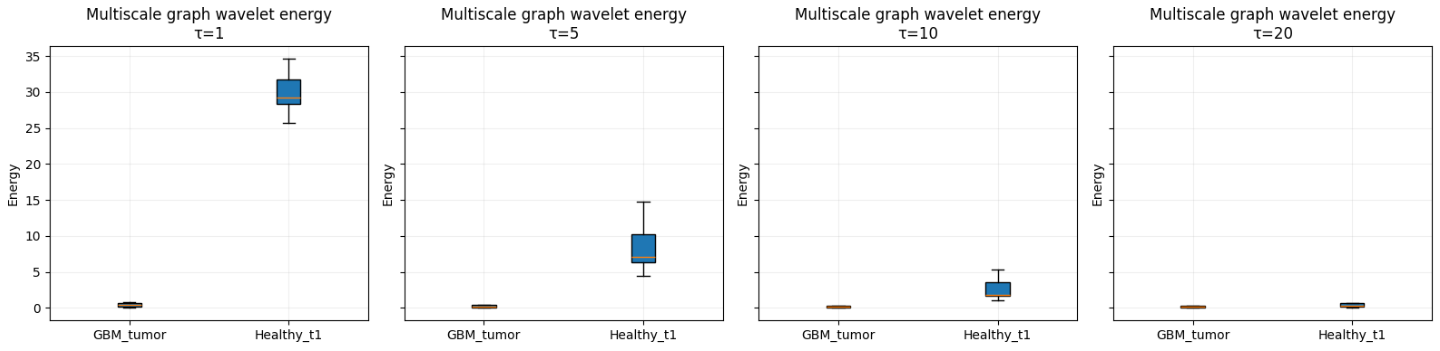
\includegraphics[width=\textwidth]{chapter4_assets/wavelet-box-whisker.png}
    \caption{Multiscale graph wavelet energy across cohorts at scales \(\tau=1,5,10,20\). The strongest group differences occur at smaller scales, where healthy T1 signals display substantially larger wavelet energy than GBM tumor signals.}
    \label{fig:wavelet_boxplots} % chktex 24
\end{figure}

\subsection{Node-wise Wavelet Coefficients}

Figure~\ref{fig:wavelet_coefficients_nodes} shows graph wavelet coefficients across nodes for a representative GBM tumor signal. The curves demonstrate how spatial detail is progressively smoothed as the scale \(\tau\) increases.

\begin{figure}[H]
    \centering
    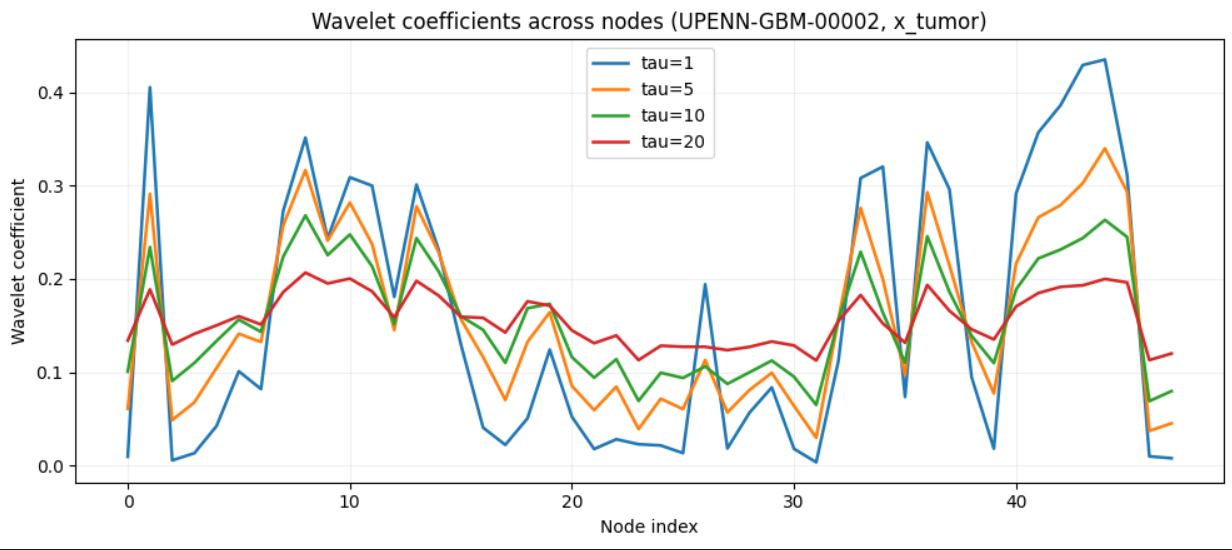
\includegraphics[width=0.92\textwidth]{chapter4_assets/wavelet-coefficients-graph.png}
    \caption{Wavelet coefficients across atlas nodes for a representative GBM tumor signal at scales \(\tau=1,5,10,20\). Small scales retain local peaks and abrupt changes; larger scales suppress these irregularities and reveal broader graph structure.}
    \label{fig:wavelet_coefficients_nodes} % chktex 24
\end{figure}

Wavelet energy is especially informative because it links directly to the smoothness prior. Signals with high fine-scale wavelet energy necessarily retain more localized irregularity on the graph, which is closely related to larger Dirichlet energy and therefore to a larger smoothness penalty in the learning objective.

\subsection{Wavelets, Smoothness, and Disease Structure}

For a spectral filter \(g\), the scale-dependent energy can be expanded as
\begin{equation}
E_{\mathrm{wav}}(\tau;x)
=
\sum_{k=1}^{N} |g(\tau\lambda_k)|^2 |\hat x_k|^2.
\end{equation}
Thus wavelet energy is simply a filtered spectral energy. It provides a useful bridge between descriptive multiscale analysis and graph-regularized learning: if the model learns node embeddings that suppress unnecessary high-frequency or fine-scale variability while keeping predictive disease patterns, then the smoothness penalty is reduced without sacrificing classification performance.

\section{Diffusion Dynamics on the Connectome}
\label{sec:ch4_diffusion} % chktex 24

\subsection{Heat Diffusion Model}

A standard physical interpretation of graph smoothness is diffusion. Let \(f(t)\in\mathbb{R}^N\) be a time-dependent graph signal satisfying
\begin{equation}
\frac{d f(t)}{dt} = -L f(t), \qquad f(0)=f_0.
\end{equation}
The solution is
\begin{equation}
\label{eq:heat_solution}
f(t)=e^{-tL}f_0 = U e^{-t\Lambda} U^\top f_0.
\end{equation}
Because each spectral component decays as \(e^{-t\lambda_k}\), high-frequency components vanish more rapidly than low-frequency ones. Diffusion therefore smooths the signal over the graph.

\subsection{Dirichlet Energy as Instantaneous Dissipation}

The derivative of the squared norm under heat diffusion is
\begin{align}
\frac{d}{dt}\|f(t)\|_2^2
&=
2 f(t)^\top \frac{d f(t)}{dt}\\ % chktex 3
&=
-2 f(t)^\top L f(t)\\ % chktex 3
&=
-2 \mathcal{E}(f(t)).
\end{align}
Hence Dirichlet energy measures the instantaneous rate at which signal energy is dissipated by diffusion. Signals with large Dirichlet energy contain sharp edge-wise discrepancies and smooth quickly; signals with small Dirichlet energy are already smooth and diffuse slowly.

\subsection{Interpretation for Brain Signals}

In the present setting, the smoothness assumption does \emph{not} mean that disease effects are spatially uniform. Rather, it imposes that the \emph{learned predictive representation} should avoid gratuitous node-to-node oscillation not supported by the graph structure. A disease focus may still induce local discontinuities; however, the model should encode these in a way that is both graph-aware and task-relevant.

This distinction is important. The objective is not to maximize smoothness at all costs, but to minimize
\[
\mathcal{L}_{\text{pred}} + \lambda \mathcal{L}_{\text{smooth}},
\]
so that the retained variation is the variation needed for discrimination.

\section{Geometric Deep Learning for Connectome Prediction}
\label{sec:ch4_gdl} % chktex 24

\subsection{Model Overview}

Given a graph \(G=(V,E,W)\) and subject signal \(x^{(s)}\), the goal is to predict whether the subject belongs to the GBM or healthy cohort. A graph neural network (GNN) is used to map node features to a graph-level representation and then to a class probability:
\begin{equation}
\hat y^{(s)} = \sigma\!\big(\phi_{\mathrm{readout}}(H^{(L,s)})\big),
\end{equation}
where \(H^{(L,s)}\in\mathbb{R}^{N\times F_L}\) is the node embedding matrix after \(L\) layers, \(\phi_{\mathrm{readout}}\) is a graph-level pooling/readout function, and \(\sigma\) is the logistic sigmoid.

The geometric deep learning workflow and training curves are summarized in Figure~\ref{fig:geometric_deep_learning}. The figure also shows the confusion matrix and the trajectory of prediction loss versus smoothness penalty during training.

\begin{figure}[H]
    \centering
    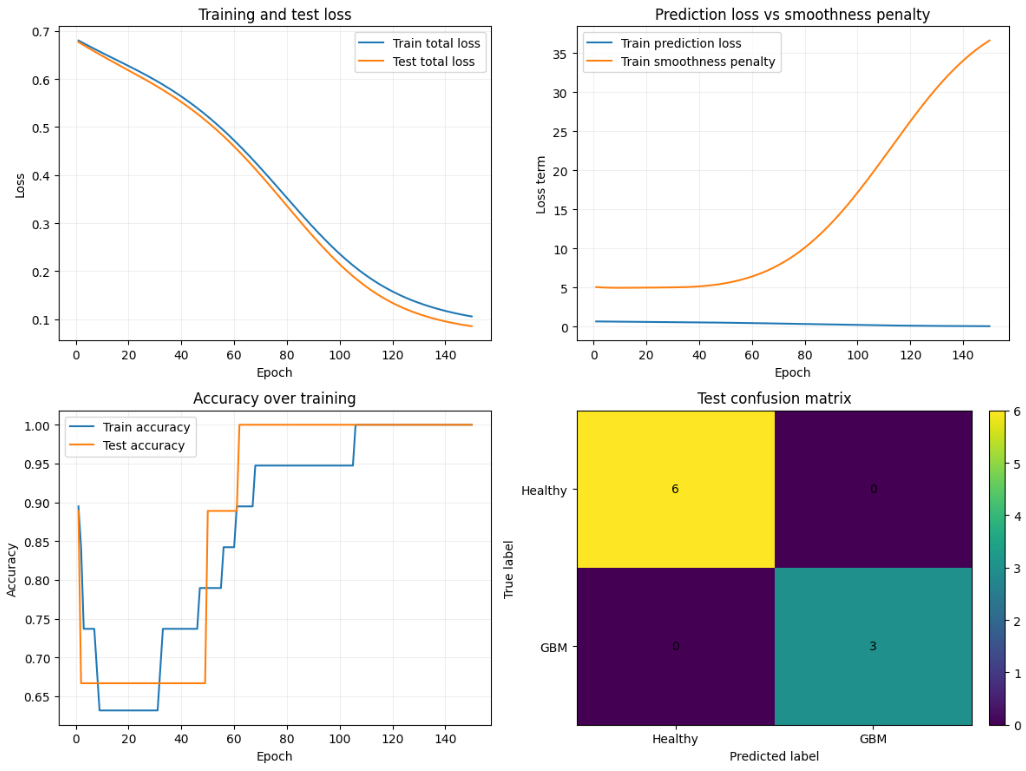
\includegraphics[width=\textwidth]{chapter4_assets/geometric-deep-learning.png}
    \caption{Geometric deep learning results. Top-left: training and test total loss curves. Top-right: evolution of the task-specific prediction loss and the smoothness penalty. Bottom-left: training and test accuracy. Bottom-right: test confusion matrix showing perfect separation on the reported split.}
    \label{fig:geometric_deep_learning} % chktex 24
\end{figure}

\subsection{Message Passing Formulation}

A standard message passing layer may be written as
\begin{equation}
h_i^{(\ell+1)}
=
\psi^{(\ell)}
\!\left(
h_i^{(\ell)},
\;
\bigoplus_{j\in\mathcal{N}(i)}
\phi^{(\ell)}(h_i^{(\ell)},h_j^{(\ell)},e_{ij})
\right),
\end{equation}
where \(h_i^{(\ell)}\) is the node embedding at layer \(\ell\), \(e_{ij}\) is an edge attribute if present, \(\phi^{(\ell)}\) computes messages, \(\oplus\) is a permutation-invariant aggregation (such as sum or mean), and \(\psi^{(\ell)}\) updates the node state.

For a graph convolution using the normalized adjacency, one may write
\begin{equation}
\label{eq:gcn_layer}
H^{(\ell+1)}
=
\rho\!\left(
\widetilde D^{-1/2}\widetilde W \widetilde D^{-1/2}
H^{(\ell)} \Theta^{(\ell)}
\right),
\end{equation}
where \(\widetilde W = W + I\), \(\widetilde D\) is its degree matrix, \(\Theta^{(\ell)}\) are learnable weights, and \(\rho\) is a pointwise nonlinearity. Equation~\eqref{eq:gcn_layer} shows explicitly how the graph topology constrains feature mixing across neighboring regions.

\subsection{Graph-Level Readout}

The graph-level embedding may be formed by global pooling:
\begin{equation}
z^{(s)} = \mathrm{READOUT}(H^{(L,s)}),
\end{equation}
for example using mean pooling
\begin{equation}
z^{(s)} = \frac{1}{N}\sum_{i=1}^{N} h_i^{(L,s)},
\end{equation}
or attention-weighted pooling
\begin{equation}
z^{(s)} = \sum_{i=1}^{N}\alpha_i^{(s)} h_i^{(L,s)}, \qquad
\sum_{i=1}^{N}\alpha_i^{(s)}=1.
\end{equation}
The output logit is then
\begin{equation}
\eta^{(s)} = w^\top z^{(s)} + b,
\end{equation}
and the predicted probability is
\begin{equation}
\hat p^{(s)} = \sigma(\eta^{(s)}) = \frac{1}{1+e^{-\eta^{(s)}}}.
\end{equation}

\subsection{Task-Specific Prediction Loss}

For binary classification, the task-specific prediction loss is the binary cross-entropy:
\begin{equation}
\label{eq:bce_loss}
\mathcal{L}_{\mathrm{pred}}
=
-\frac{1}{M}\sum_{s=1}^{M}
\left[
y^{(s)}\log \hat p^{(s)} + \big(1-y^{(s)}\big)\log\big(1-\hat p^{(s)}\big)
\right],
\end{equation}
where \(M\) is the number of training subjects.

\subsection{Smoothness Penalty Based on Dirichlet Energy}

To encourage graph-consistent node embeddings, the smoothness penalty is defined using the Dirichlet energy of a learned representation. Let \(H^{(L,s)}=[h_1^{(L,s)},\dots,h_N^{(L,s)}]^\top\in\mathbb{R}^{N\times F}\). A natural matrix-valued generalization of graph Dirichlet energy is % chktex 3
\begin{equation}
\label{eq:matrix_dirichlet}
\mathcal{E}\!\big(H^{(L,s)}\big)
=
\mathrm{Tr}\!\left((H^{(L,s)})^\top L H^{(L,s)}\right) % chktex 3
=
\frac{1}{2}\sum_{i,j}W_{ij}\|h_i^{(L,s)}-h_j^{(L,s)}\|_2^2.
\end{equation}
Averaging over the training batch gives
\begin{equation}
\label{eq:smoothness_loss}
\mathcal{L}_{\mathrm{smooth}}
=
\frac{1}{M}\sum_{s=1}^{M}
\mathrm{Tr}\!\left((H^{(L,s)})^\top L H^{(L,s)}\right). % chktex 3
\end{equation}
This is the smoothness term used in the overall objective
\begin{equation}
\label{eq:full_training_objective}
\mathcal{L}_{\mathrm{total}}
=
\mathcal{L}_{\mathrm{pred}}
+
\lambda \mathcal{L}_{\mathrm{smooth}}.
\end{equation}
Expanding Equation~\eqref{eq:smoothness_loss} shows directly what is penalized:
\begin{equation}
\mathcal{L}_{\mathrm{smooth}}
=
\frac{1}{2M}\sum_{s=1}^{M}\sum_{i,j}W_{ij}
\|h_i^{(L,s)} - h_j^{(L,s)}\|_2^2.
\end{equation}
Thus neighboring nodes with strong graph affinity are encouraged to have similar final embeddings unless task-specific gradients force them apart.

\subsection{Gradient Interpretation}

If one differentiates the smoothness term with respect to \(H^{(L,s)}\), the result is
\begin{equation}
\frac{\partial}{\partial H^{(L,s)}}
\mathrm{Tr}\!\left((H^{(L,s)})^\top L H^{(L,s)}\right) % chktex 3
=
2L H^{(L,s)}.
\end{equation}
Hence the smoothness gradient acts as a graph diffusion operator on the learned node embeddings. The optimizer therefore balances:
\begin{enumerate}[label=(\arabic*)] % chktex 36
    \item the discriminative gradient from \(\mathcal{L}_{\mathrm{pred}}\), which preserves class-separating information, and
    \item the smoothing gradient from \(\mathcal{L}_{\mathrm{smooth}}\), which suppresses unnecessary graph-inconsistent fluctuations.
\end{enumerate}

\subsection{Training Dynamics}

The training curves in Figure~\ref{fig:geometric_deep_learning} reveal three important patterns:
\begin{enumerate}[label=(\alph*)] % chktex 36
    \item the total loss decreases smoothly on both train and test sets;
    \item classification accuracy improves to perfect separation on the reported split;
    \item the smoothness penalty increases as training proceeds, while the prediction loss decreases.
\end{enumerate}
The third pattern is particularly informative: to improve discrimination, the model learns embeddings that are less smooth than the initialization. This is not contradictory. The objective does not minimize smoothness alone; it minimizes the \emph{sum} of a task loss and a smoothness penalty. As a result, the optimum may legitimately move toward a higher smoothness term when that increase is more than compensated by a larger reduction in \(\mathcal{L}_{\mathrm{pred}}\).

This behavior is fully consistent with Equation~\eqref{eq:full_training_objective}. The regularizer does not prohibit task-relevant graph variation; rather, it discourages gratuitous variation. In other words, the model is allowed to pay a smoothness cost to represent clinically meaningful disease contrast.

\subsection{Performance Summary}

The test confusion matrix in Figure~\ref{fig:geometric_deep_learning} shows \(6/6\) healthy and \(3/3\) GBM examples correctly classified on the reported split. The PCA projection of learned subject embeddings further demonstrates class separation.

\begin{figure}[H]
    \centering
    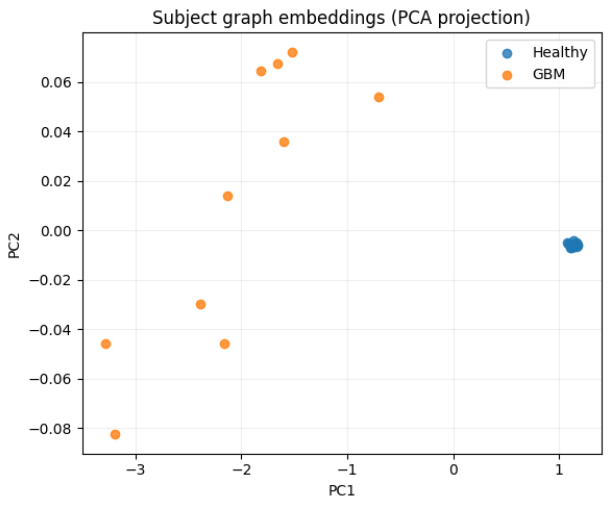
\includegraphics[width=0.62\textwidth]{chapter4_assets/pca-projection.png}
    \caption{PCA projection of learned subject embeddings. Healthy subjects form a compact cluster, while GBM subjects occupy a well-separated region of the embedding space, indicating that the learned representation is highly discriminative.}
    \label{fig:pca_projection} % chktex 24
\end{figure}

Table~\ref{tab:training_objective_summary} summarizes the components of the training objective.

\begin{table}[H]
    \centering
    \caption{Training objective components and interpretations.}
    \label{tab:training_objective_summary} % chktex 24
    \begin{tabular}{p{3.6cm} p{5.2cm} p{6.2cm}}
        \toprule
        \textbf{Component} & \textbf{Formula} & \textbf{Purpose} \\
        \midrule
        Prediction loss &
        \(\mathcal{L}_{\mathrm{pred}}
        =-\frac{1}{M}\sum_s \big[y^{(s)}\log \hat p^{(s)}+(1-y^{(s)})\log(1-\hat p^{(s)})\big]\) &
        Encourages accurate subject-level disease classification. This is the task-specific term. \\
        \addlinespace
        Smoothness penalty &
        \(\mathcal{L}_{\mathrm{smooth}}
        =\frac{1}{M}\sum_s \mathrm{Tr}\big((H^{(L,s)})^\top L H^{(L,s)}\big)\) & % chktex 3
        Penalizes edge-wise discrepancies in learned node embeddings, encouraging graph-consistent representations. \\
        \addlinespace
        Total objective &
        \(\mathcal{L}_{\mathrm{total}}
        = \mathcal{L}_{\mathrm{pred}}+\lambda \mathcal{L}_{\mathrm{smooth}}\) &
        Balances classification performance against graph-structured regularity. \\
        \bottomrule
    \end{tabular}
\end{table}

\section{Spectral Biomarkers of Disease}
\label{sec:ch4_biomarkers} % chktex 24

The descriptive analyses suggest that disease and healthy cohorts differ in how signal energy is distributed over graph frequencies and graph scales. These differences support the following candidate biomarkers:

\subsection{Spectral Centroid as a Compact Frequency Summary}

From Equation~\eqref{eq:spectral_centroid}, the spectral centroid quantifies where the graph signal ``lives'' along the frequency axis. In the present dataset, healthy T1 signals tend to have larger centroids than GBM T1 signals (Figures~\ref{fig:centroid_box} and \ref{fig:centroid_box_all}), indicating a shift toward higher graph frequencies. % chktex 2

\subsection{High-Frequency Energy as an Irregularity Measure}

The high-frequency energy \(E_{\mathrm{high}}\) is a direct proxy for graph-local irregularity. In the cohort comparisons of Figures~\ref{fig:highfreq_box} and \ref{fig:highfreq_box_all}, healthy signals occupy a higher range than GBM-related signals, suggesting more distributed and less low-frequency-dominated graph structure in the healthy cohort. % chktex 2

\subsection{Spectral Entropy as a Complexity Measure}

The entropy measure of Equation~\eqref{eq:spectral_entropy} is highest for the healthy cohort (Figure~\ref{fig:entropy_box}). This implies that healthy graph signals spread their energy over a wider range of modes, whereas disease-related signals are relatively more concentrated. Such compression may arise when disease burden occupies a more localized subnetwork or when pathology suppresses broad variability.

\subsection{Wavelet Energy as a Multiscale Biomarker}

Wavelet energy distinguishes cohorts at fine and intermediate scales (Figure~\ref{fig:wavelet_boxplots}), complementing purely spectral summaries. This suggests that disease-related changes are not only frequency-specific but also scale-specific on the graph.

\subsection{Interpretive Synthesis}

Taken together, the figures suggest the following pattern:
\begin{itemize}
    \item GBM tumor signals are more concentrated in lower graph frequencies;
    \item healthy T1 signals exhibit higher spectral centroid, higher entropy, and higher high-frequency energy;
    \item multiscale wavelet energy is largest in healthy signals, especially at smaller scales;
    \item disease effects are localized over specific atlas nodes and subnetworks rather than uniformly distributed.
\end{itemize}

These observations justify using graph-structured regularization in a classifier: the graph carries biologically meaningful spatial organization, and the spectrum provides an interpretable basis for quantifying disease-related departures from typical organization.

\section{Stability and Robustness Considerations}
\label{sec:ch4_robustness} % chktex 24

The methodology combines a fixed shared graph with subject-varying signals. This setup offers several stability advantages:
\begin{enumerate}[label=(\arabic*)] % chktex 36
    \item \textbf{Common node semantics:} every node corresponds to the same atlas region across subjects;
    \item \textbf{Shared spectral basis:} the eigenvectors of the common graph provide a single reference frame for all graph Fourier analyses;
    \item \textbf{Regularized learning:} the Dirichlet penalty reduces the risk of overfitting to noisy subject-specific node fluctuations.
\end{enumerate}

If the observed signal is \(x = x^\star + \varepsilon\), where \(\varepsilon\) is noise, then
\begin{equation}
\mathcal{E}(x)
=
\mathcal{E}(x^\star)
+
2(x^\star)^\top L \varepsilon % chktex 3
+
\mathcal{E}(\varepsilon).
\end{equation}
Noise concentrated at high graph frequencies inflates the Dirichlet energy because
\begin{equation}
\mathcal{E}(\varepsilon)=\sum_{k=1}^{N}\lambda_k |\hat\varepsilon_k|^2.
\end{equation}
Thus the smoothness penalty preferentially suppresses high-frequency noise. In this sense, graph regularization has a denoising interpretation as well as a structural prior interpretation.

At the model level, the parameter \(\lambda\) controls a bias--variance tradeoff: % chktex 8
\begin{itemize}
    \item if \(\lambda\) is too small, the model may overfit node-wise idiosyncrasies;
    \item if \(\lambda\) is too large, the model may oversmooth embeddings and suppress clinically meaningful local abnormalities.
\end{itemize}
The training dynamics in Figure~\ref{fig:geometric_deep_learning} suggest that the chosen setting permits strong predictive separation while still imposing a meaningful graph prior.

\section{Results Overview}
\label{sec:ch4_results_overview} % chktex 24

The empirical results can be summarized along three complementary axes.

\subsection{Axis I: Spatial Organization on the Graph} % chktex 13

Figures~\ref{fig:connectome_descriptive_statistics}, \ref{fig:gbm_mean_presence}, \ref{fig:mean_signal_graphs}, and \ref{fig:tumor_by_node} show that both tumor burden and image-derived signals possess clear spatial organization on the shared connectome. Disease involvement is concentrated in subsets of atlas nodes and manifests as structured regional deviations. % chktex 2

\subsection{Axis II: Spectral and Multiscale Separation} % chktex 13

Figures~\ref{fig:cancer_vs_normal_spectra}--\ref{fig:highfreq_box_all} and \ref{fig:wavelet_boxplots} demonstrate consistent group differences in graph spectral descriptors and multiscale wavelet energy. These results indicate that disease can be detected not only in the spatial domain but also in the graph frequency domain. % chktex 2

\subsection{Axis III: Predictive Learning Under Graph Regularization} % chktex 13

Figures~\ref{fig:geometric_deep_learning} and \ref{fig:pca_projection} show that a geometric deep learning model regularized by graph smoothness can produce a strongly discriminative embedding space. The class separation in PCA space and the perfect confusion matrix on the reported split suggest that the learned representation captures robust disease-related structure. % chktex 2

\subsection{Consolidated Interpretation}

The chapter's central conclusion is that connectome-aware analysis is valuable both descriptively and predictively. Descriptively, the graph Fourier basis and graph wavelets reveal where disease-related information is located across graph frequencies and scales. Predictively, the same graph supports a smoothness-regularized learning objective:
\[
\mathcal{L}_{\mathrm{total}}
=
\mathcal{L}_{\mathrm{pred}}
+
\lambda \mathcal{L}_{\mathrm{smooth}}.
\]
This objective is principled because it reflects the assumption that neighboring brain regions should generally have related latent representations, except where the classification task benefits from preserving edge-wise contrast.

\section{Discussion}
\label{sec:ch4_discussion} % chktex 24

This chapter established a full graph signal processing pipeline for atlas-based brain connectome analysis. The main contributions are:
\begin{enumerate}[label=(\arabic*)] % chktex 36
    \item a shared 48-node atlas graph representation for all subjects,
    \item graph signal definitions for T1 intensity and tumor burden,
    \item spectral biomarkers including high-frequency energy, spectral centroid, and spectral entropy,
    \item multiscale graph wavelet analysis of disease-related signals,
    \item a diffusion-based interpretation of smoothness via Dirichlet energy, and
    \item a geometric deep learning classifier trained under a smoothness-regularized objective.
\end{enumerate}

A particularly important conceptual result is the role of the smoothness regularizer. Because it is derived from Dirichlet energy,
\[
\mathcal{L}_{\mathrm{smooth}}
=
\frac{1}{M}\sum_{s=1}^{M}
\mathrm{Tr}\!\left((H^{(L,s)})^\top L H^{(L,s)}\right), % chktex 3
\]
it directly penalizes graph-inconsistent variation in learned node embeddings. However, the total objective remains
\[
\mathcal{L}_{\mathrm{total}}
=
\mathcal{L}_{\mathrm{pred}}
+
\lambda \mathcal{L}_{\mathrm{smooth}},
\]
so the model preserves irregularity when that irregularity is informative for class discrimination. The increasing smoothness term during training is therefore not a failure of the regularizer; it is evidence that the optimization is balancing task-specific discrimination against graph-based prior structure exactly as intended.

In summary, the results support the view that disease-related brain patterns are best understood as graph signals over a biologically meaningful network. The combination of spectral analysis, graph wavelets, and smoothness-regularized geometric learning provides a coherent framework for both mechanistic interpretation and accurate prediction.

\FloatBarrier % chktex 1

% ------------------------------------------------------------------
% Optional appendix-style compact notation table for this chapter
% ------------------------------------------------------------------
\begin{table}[H]
    \centering
    \caption{Compact notation summary for Chapter~\ref{chap:gsp_connectome}.}
    \label{tab:notation_ch4} % chktex 24
    \begin{tabular}{p{2.6cm} p{11.8cm}}
        \toprule
        \textbf{Symbol} & \textbf{Meaning} \\
        \midrule
        \(G=(V,E,W)\) & Weighted undirected connectome graph with node set \(V\), edge set \(E\), and adjacency matrix \(W\). \\
        \(N\) & Number of graph nodes (here \(N=48\)). \\
        \(D\) & Degree matrix, \(D_{ii}=\sum_j W_{ij}\). \\
        \(L\) & Combinatorial graph Laplacian, \(L=D-W\). \\
        \(L_{\mathrm{sym}}\) & Symmetric normalized Laplacian, \(I-D^{-1/2}WD^{-1/2}\). \\
        \(x^{(s)}\) & Graph signal for subject \(s\). \\
        \(\hat x\) & Graph Fourier transform of \(x\), \(\hat x = U^\top x\). \\
        \(U,\Lambda\) & Laplacian eigenvectors and eigenvalues, with \(L=U\Lambda U^\top\). \\
        \(\mathcal{E}(x)\) & Dirichlet energy, \(x^\top L x\). \\
        \(E_{\mathrm{high}}\) & High-frequency spectral energy. \\
        \(C_{\mathrm{spec}}\) & Spectral centroid. \\
        \(H_{\mathrm{spec}}\) & Spectral entropy. \\
        \(H^{(L,s)}\) & Final-layer node embedding matrix for subject \(s\). \\
        \(\mathcal{L}_{\mathrm{pred}}\) & Task-specific prediction loss (binary cross-entropy). \\
        \(\mathcal{L}_{\mathrm{smooth}}\) & Smoothness penalty based on Dirichlet energy of learned embeddings. \\
        \(\lambda\) & Regularization strength balancing prediction and smoothness. \\
        \bottomrule
    \end{tabular}
\end{table}